
%(BEGIN_QUESTION)
% Copyright 2014, Tony R. Kuphaldt, released under the Creative Commons Attribution License (v 1.0)
% This means you may do almost anything with this work of mine, so long as you give me proper credit

Les og lag disposisjon av delseksjonen ``Instrumentation Amplifiers'' og introduksjonen til seksjonen ``Analog Signal Conditioning and Referencing'' i kapittelet ``Digital Data Acquisition and Networks'' i læreboken {\it Lessons In Industrial Instrumentation}. Noter sidetall for viktige illustrasjoner, fotografier, ligninger, tabeller og andre relevante detaljer. Forbered deg på å diskutere begreper og eksempler fra lesingen med lærer og medstudenter.

\underbar{file i00882}
%(END_QUESTION)





%(BEGIN_ANSWER)


%(END_ANSWER)





%(BEGIN_NOTES)

Problem som må løses: hvordan tilpasse inngangsområdet til ADC-en til et gitt virkelig spenningssignal? Hvis signalet er for stort, kan vi bruke en motstandsbasert spenningsdeler for å redusere signalet ned til ADC-området. Hvis signalet er for lite, utnyttes ikke ADC-ens telleområde effektivt. Vi må ``kondisjonere'' signalet slik at det passer ADC-ens inngangskrav.

\vskip 10pt

Et annet problem: inkompatible jordreferanser. Noen ganger kan vi ikke koble én side av et virkelig signal til jord uten alvorlige problemer, som kortslutninger. Lar vi ADC-en ``flyte'' på forhøyet potensial, oppstår problemer på digitalbuss-siden fordi common-mode-spenningen forstyrrer korrekt tolkning av bitnivåer. En differensialforsterker som tåler common-mode-spenning på inngangene løser dette ved å ``flytte'' signalets common-mode-spenning til null, altså oversette et ``flytende'' differensialsignal til et jordreferert signal ADC-en kan håndtere. En differensialforsterker kan også forsterke svake signaler ved behov. Også dette er en form for ``kondisjonering'' før digitalisering.

\vskip 10pt

En ``instrumentation amplifier'' er en spesiell differensialforsterker med buffrede innganger (høy inngangsimpedans) og forsterkning styrt av én ekstern motstand. Forsterkningen kan typisk justeres mellom 1 og uendelig. DAQ-moduler har vanligvis én slik forsterker per inngangskanal.






\vskip 20pt \vbox{\hrule \hbox{\strut \vrule{} {\bf Forslag til sokratisk diskusjon} \vrule} \hrule}

\begin{itemize}
\item{} Forklar hva {\it common-mode}-spenning er, og hvorfor det kan være et problem i datainnsamling.
\item{} Finn en løsning for måling av både solpanelspenning og laststrøm som {\it ikke} krever instrumentation amplifier. Hint: flytt shuntmotstanden.
\item{} Hvor høye må forsyningsskinnene være for differensialforsterkerkretsen i teksten for å håndtere 33 V ut fra solpanelet?
\item{} Hvor praktisk er det å bruke større shuntmotstand i stedet for differensialforsterker {\it med gain} for bedre utnyttelse av ADC-spenningsområdet?
\item{} Forklar hvorfor gain for instrumentation amplifier øker når $R_G$ reduseres, ut fra kretsen (ikke bare formelen). Strategien ``grensetilfeller'' kan være nyttig.
\item{} Forklar hensikten med ``MUX'' i en DAQ-modul. Hvorfor trenger vi en multiplekser i en datainnsamlingsenhet?
\item{} I ``final solution''-diagrammet med 4-kanals DAQ koblet til solpanelkretsen: er 10:1-spenningsdeleren fortsatt nødvendig? Forklar.
\item{} I samme ``final solution''-diagram: hvilken kanal bør settes med størst {\it gain}? Krever dette stor eller liten $R_G$?
\end{itemize}






\vfil \eject

Beregn alle spenningsfall og strømmer gitt $V_{panel}$, $I_{load}$ og verdi for alle motstander ($R$) i denne kretsen:

$$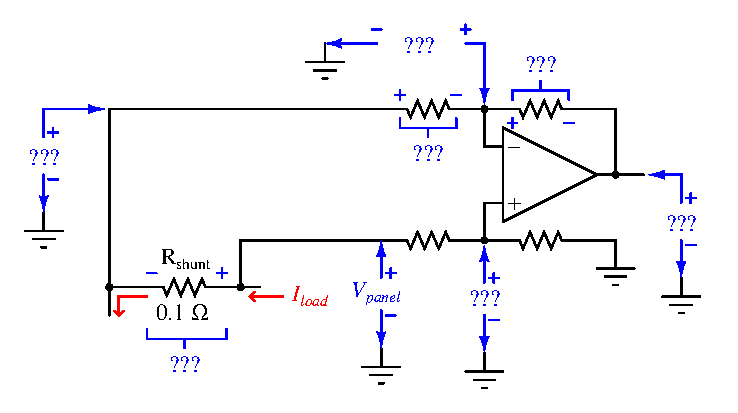
\includegraphics[width=15.5cm]{i00882x01.eps}$$








\vfil \eject

\noindent
{\bf Forberedende quiz:}

Forklar hva {\it common-mode}-spenning er. Vær så konkret som mulig, og bruk gjerne en realistisk applikasjon i forklaringen.









\vfil \eject

\noindent
{\bf Forberedende quiz:}

Beskriv hvordan du endrer gain i en {\it instrumentation amplifier}. Vær så konkret som mulig, og bruk gjerne en realistisk applikasjon i forklaringen.



%INDEX% Reading assignment: Lessons In Industrial Instrumentation, Digital Data Acquisition and Networks (instrumentation amplifiers)

%(END_NOTES)
